% !TeX spellcheck = da_DK
\documentclass[12pt,fleqn]{article}

\usepackage[danish]{babel}
\usepackage{SpeedyGonzales}
\usepackage{MediocreMike}
%\usepackage{Blastoise}

\title{}
\author{Asger Schultz}
\date{\today}

\fancypagestyle{plain}
{
	\fancyhf{}
	\rfoot{Side \thepage{} af \pageref{LastPage}}
	\renewcommand{\headrulewidth}{0pt}
}
\pagestyle{fancy}
\fancyhf{}
\lhead{Asger Schultz}
\chead{}
\rhead{}
\rfoot{Side \thepage{} af \pageref{LastPage}}

\graphicspath{{Billeder/}}
\linespread{1.15}


%\numberwithin{equation}{section}
%\numberwithin{footnote}{section}
%\numberwithin{figure}{section}
%\numberwithin{table}{section}

\begin{document}

\maketitle
%\thispagestyle{fancy}
%\tableofcontents

\section{Data}
\begin{itemize}
	\item Experiment 4
	\item 10 -People: 10 Repetitions
	\item Each repetition: 100 3D-coordinates
\end{itemize}

\section{Machine Learning task}
\subsection{The task: Classification}
\begin{itemize}
\item For machine learning: Consider data as a 10-class (person) problem with 10 observations (repetitions) each consisting of 300 features 
\item High dimensional 10-class classification 
\item Plot: Seems nonlinear (parabolic data)
\end{itemize}
\begin{figure}[H]
	\centering
	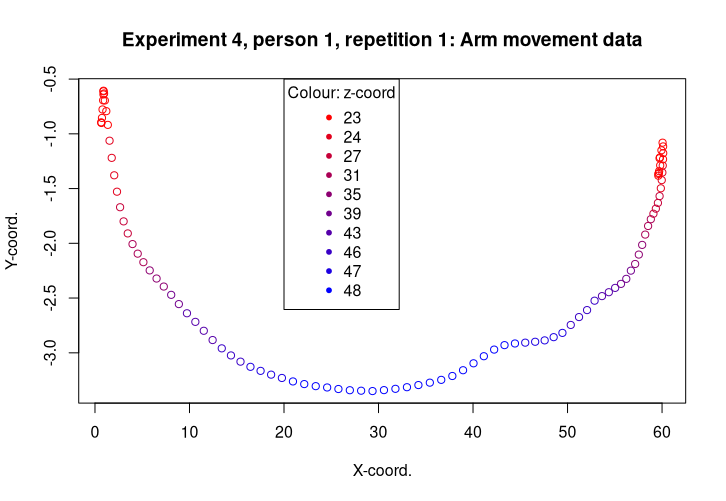
\includegraphics[width=.7\linewidth]{p1_example}
\end{figure}
\subsection{Models and training}
\begin{itemize}
	\item Considers non-linear models
	\item KNN:
	\item Classification trees: Hunt's algorithm
	\item Baseline: 10\pro
\end{itemize}
\subsection{Performance evaluation}
\begin{itemize}
	\item Complexity-controlling parameters
	\item Leave-one-out crossvalidation
	\item McNemar's test
\end{itemize}
\section{Test of experiment effect}
\begin{itemize}
	\item Expectation: Yes, significant difference as 15 different obtacle avoidance tests + control is considered
\end{itemize}
\begin{itemize}
	\item Introduce ANOVA: Model assumptions
	\item Introduce factors
\end{itemize}
\begin{figure}[H]
	\centering
	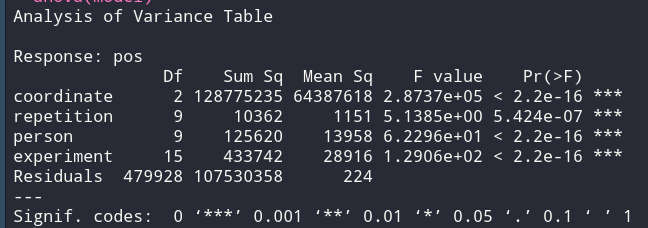
\includegraphics[width=.7\linewidth]{p1_anova}
\end{figure}
\begin{itemize}
	\item Yes, experiment is significant. 
	\item Surprise: Repetition is also significant though
	\item Which coordinate it is explains the largest part of data variability but experiment no. comes in second
	\item Low residual variance when compared to within-group variance
\end{itemize}
\begin{figure}[H]
	\centering
	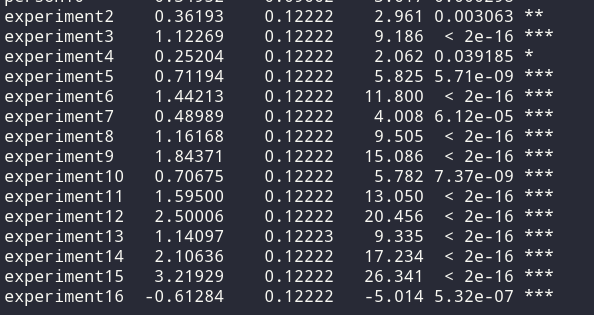
\includegraphics[width=.7\linewidth]{p1_anova_summay}
\end{figure}
\end{document}

















